\documentclass[]{article} %la classe mi preimposta alcune opzioni 
\usepackage{subfiles}
%latex packages
%
% ------------------PACKAGES
% 
\usepackage{graphicx} %per inserire figure
\usepackage{enumerate} %per liste numerate, mettere * quando non voglio il nr
\usepackage{wrapfig} % raggruppare una figura e poterne gestire meglio il posizionamento
\usepackage{comment} % mi permette di commentare più linee
\usepackage{csquotes} %for quotations
\usepackage{blindtext} %for random text

\usepackage{tikz} % for drawing lines
%\newtheorem{definition}{printed def} % può essere utile per le definizioni
%\newtheorem*{remark}{nota}
\usepackage{lmodern} %in alternativa lmodern, palatino, times, helvet
\usepackage[dvipsnames]{xcolor} %per una gestioen più ampia dei colori, lopzione tra [] mi da più ampia scelta di colori find other colors here https://www.overleaf.com/learn/latex/Using_colors_in_LaTeX
%\usepackage[scaled]{beramono} %resets the monospace font in the document
\usepackage{dialogue} % per i dialoghi
\usepackage{fancybox} %per caselle di testo

\definecolor{MyCustomColor}{RGB}{198,162,1}
\definecolor{NewColor}{HTML}{665544}
%
\usepackage{multicol} % Essential for multi-column layouts

% Other useful packages (explained later)
\usepackage{lipsum}  % For generating filler text
\usepackage[margin=0.75in, a4paper]{geometry} % To control page margins
\usepackage{fancyhdr} % For custom headers/footers
\usepackage{exsheets} %for exercises 
\pagestyle{fancy}


\lhead{Lesson 5 - Ist. Mandes - Casalnuovo} % Left header content
\rhead{Travel}   % Right header content
\rfoot{13/05/2024}


\begin{document}
	
\section*{Reading and writing}

\begin{question}
	\textbf{Read the following text and identify which writing style it is applied: Letter, Article or Essay}
\end{question}	


\subsection*{Letter, Article or Essay?}

\subsubsection*{Traveling Makes You Smarter}

Did you know traveling can help you do better in school? It's true! When you visit a new place, you learn about different cultures, see amazing things, and maybe even try speaking a new language. This makes your brain work in new ways. Traveling helps you become more curious and open-minded. It can even improve your math skills (figuring out money exchange) and reading skills (learning new signs). So, next time you're planning a family trip, remember – it's not just fun, it's an adventure for your brain!

\begin{wrapfigure}{r}{0.5\textwidth}
	\raggedleft
	\includegraphics[width=0.4\textwidth]{/home/ada/Nextcloud2/risorse-next/istockphoto-879119654-1024x1024-mongolfiera.jpg}
	\caption {Hot air balloon in Cappadocia (Turkey)}
\end{wrapfigure}

\subsubsection*{Why I Love to Travel}

Traveling is like opening a magical door to a whole new world. I love trying foods that I've never tasted before, even if they seem a bit strange at first. It's amazing to see buildings that are hundreds of years old or mountains that touch the clouds. The best part of traveling is meeting new people. Even if we don't speak the same language, we can still laugh together and share our stories. Traveling makes me realize the world is so big and exciting, and I'm just a small part of it all.



\subsubsection*{Dear Grandma}

Guess what? I'm going on a school trip to London! I'm a little nervous but mostly super excited. We're going to learn about the rise and the importance of the capital of the UK throughout history. I promise to take lots of pictures to show you. Maybe next summer, we can go on a trip together! What's your favorite place you've ever visited?

Love,
[Your name] \par 
\vspace{1cm}

\begin{minipage}[h]{0.9\textwidth}	
	
	\begin{multicols}{2}
		
		
		
		\shadowbox{
			\large{WRITING STYLES}
		}
		
		\centering
		\subsubsection*{Article}
		
		\begin{itemize}
			\item{Informative: Focuses on delivering facts and information.}
			\item{Impersonal: Avoids using "I" or addressing the reader directly. Maintains a neutral tone.}
			\item{Structured: Typically has clear headings and short paragraphs for easy reading.}
			\item{Vocabulary: Might use slightly more complex words, since the goal is to teach and expand knowledge.}
		\end{itemize}
		
		\subsubsection*{Essay}
		
		\begin{itemize}
			\item{Personal: Expresses the writer's own thoughts and feelings (uses "I").}
			\item{Reflective: Goes beyond just stating facts, explores a theme or idea.}
			\item{Creative: Can use more descriptive language and imagery than an article.}
			\item{Flow: Ideas connect smoothly, making it read like a mini-story.}
		\end{itemize}
		
		\subsubsection*{Letter}
		\begin{itemize}
			\item{Direct Address: Speaks directly to the reader ("you", in this case the grandma)}
			\item{Informal: Conversational tone, like you're chatting with a friend.}
			\item{Personal details: Includes specific feelings and plans. Might even ask questions to keep the conversation going.}
			\item{Simple language: Uses easy-to-understand vocabulary, suited for the age level.}
		\end{itemize}
		
	\end{multicols}
\end{minipage}

\newpage

\begin{question}
	\textbf{Choose one of the following opinion and write about them using either the style of a letter, an article or an essay.}
\end{question}	

\vspace{1cm}
\begin{minipage}[h]{0.95\textwidth}
	
	
	\subsection*{Four Opinions, One Discussion. Let's Go!}
	\begin{dialogue}
		
		
		\speak{Sally} I absolutely love immersing myself in different cultures when I travel. One time,
		I was in India and decided to try street food that I had never seen before. It was a
		bit intimidating at first, but it ended up being the most delicious meal I had on
		the whole trip! \par 
		\speak{Dave} I'm not a fan of straying off the tourist path and trying new things. When I was in
		France, I only stuck to the popular tourist spots and restaurants recommended in
		guidebooks. I prefer to play it safe and stick to what I know. \par 
		
		\speak{Emma} I can't decide if I should fully embrace local cultures when I travel or not. On one
		hand, I love trying new things and interacting with locals like I did in Thailand. But
		on the other hand, I also enjoy the comfort of sticking to familiar routines and
		foods. \par 
		\speak{Jack} Experiencing different cultures is so important to me. When I was in Japan, I felt
		a deep connection to the people and their way of life. I remember visiting a
		traditional tea ceremony and being moved to tears by the beauty and simplicity
		of the ritual. \par 
		
	\end{dialogue}
	
	
\end{minipage}

\vspace{1cm}




\section*{Vocabulary}

\begin{minipage}[h]{0.7\textwidth}
	\begin{center}
		
		\begin{tabular}{ p{3.5cm} p{3.5cm} p{3.5cm} p{3.5cm}}
			
			
			%**Travel Essentials**
			
			Travel (verb)
			& Trip
			& Luggage / Baggage
			& Passport
			\vfil	\\ Ticket
			& Currency
			& Transportation
			
			%**Modes of Transportation**
			
			& Airplane/Plane
			\\ Train
			& Bus
			& Taxi/Cab & Lost
			\vfil	\\ Departure
			& Arrival
			
			%**Accommodation*
			
			& Hotel
			& Hostel
			\\ Resort
			& Check-in
			& Check-out
			
			%*Sightseeing**
			
			& Landmark
			\\ Museum
			& Tour
			& Souvenir
			
			%*Additional Useful Terms**
			& Adventure
			\\ Explore
			& Foreign
			& Customs
			& Map \\
		
			
			
		\end{tabular}
		
	\end{center}
	
\end{minipage}

\subsection*{}
\begin{question}
	\textbf{Make Sentences from These Words!}
\end{question}

\begin{wrapfigure}{r}{0.5\textwidth}
	\raggedleft
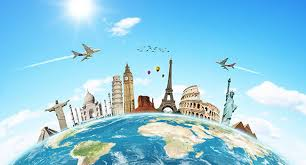
\includegraphics[width=0.45\textwidth]{/home/ada/Nextcloud2/risorse-next/mandes-esperto/english-movers_gitrepo/world-travel.jpeg}

\end{wrapfigure}


Considered / traveling / country \par
Learning / basic / phrases \par
Exploring / local / markets \par
Trying / traditional / dishes \par
Prefer / staying / hostels \par
Meeting / locals / unique \par
Planning / itinerary / advance \par
Visiting / historical / sites \par
Tried / adventurous / activities \par
Keeping / open / mind \par

\subsection*{}
\begin{question}
	\textbf{Match these words and phrases to their translations!}
\end{question}

\begin{centering}
	\begin{tabular}{ l @{\hspace{3cm}} l}
		Passport & Dogana \\
		Check-out& Passaporto \\
		Train& Mappa \\
		Landmark& Albergo \\
		Hotel&Esplorare \\
		Tour&Partenza \\
		Museum&Punto di riferimento \\
		Resort&Perso \\
		Explore&Biglietto \\
		Bus&Treno \\
		Souvenir&Check-out \\
		Customs&Museo \\
		Departure&Straniero \\
		Map&Viaggio \\
		Foreign&Souvenir \\
		Ticket&Resort \\
		Lost&Avventura \\
		Arrival&Arrivo \\
		Trip&Autobus \\
		Adventure&Tour \\
	\end{tabular}
	
\end{centering}


\subsection*{}

\begin{question}
	\textbf{Can You Find the Right Word Form?}
\end{question}


\begin{enumerate}
	
	
	\item{I am planning a \tikz \draw[dashed] (0,0) -- (5,0);(tripping) to the beach next month.}
	\item{Don't forget to bring your \tikz \draw[dashed] (0,0) -- (5,0);(pass) when travelling abroad.}
	\item{I bought my \tikz \draw[dashed] (0,0) -- (5,0);(tick) for the concert online yesterday.}
	\item{We will take the \tikz \draw[dashed] (0,0) -- (5,0);(training) to London for our holiday.}
	\item{Let's catch the \tikz \draw[dashed] (0,0) -- (5,0);(busing) to the city centre this afternoon.}
	\item{The \tikz \draw[dashed] (0,0) -- (5,0);(depart) time for our flight is early in the morning.}
	\item{Our \tikz \draw[dashed] (0,0) -- (5,0);(arrive) at the hotel was delayed due to traffic.}
	\item{We booked a room at a luxurious \tikz \draw[dashed] (0,0) -- (5,0);(hostel) by the beach.}
	\item{The \tikz \draw[dashed] (0,0) -- (5,0);(resorting) we stayed at had a beautiful swimming pool.}
	\item{Remember to \tikz \draw[dashed] (0,0) -- (5,0);(checking-out) before 12 pm on the last day.}
	\item{The Eiffel Tower is a famous \tikz \draw[dashed] (0,0) -- (5,0);(landmarker) in Paris.}
	\item{We visited the \tikz \draw[dashed] (0,0) -- (5,0);(muse) to learn about ancient history.}
	\item{Joining a guided \tikz \draw[dashed] (0,0) -- (5,0);(touring) of the city can be very informative.}
	\item{I bought a lovely \tikz \draw[dashed] (0,0) -- (5,0);(souvenirize) from the gift shop.}
	\item{Travelling to new places always brings excitement and \tikz \draw[dashed] (0,0) -- (5,0);(adventuring).}
	\item{Let's \tikz \draw[dashed] (0,0) -- (5,0);(explorer) the old town and discover hidden gems.}
	\item{Trying \tikz \draw[dashed] (0,0) -- (5,0);(foreigner) cuisine is one of the best parts of travelling.}
	\item{Passing through \tikz \draw[dashed] (0,0) -- (5,0);(custom) can sometimes be a lengthy process.}
	\item{Can you show me where we are on the \tikz \draw[dashed] (0,0) -- (5,0);(mapping)?}
	\item{Be careful not to get \tikz \draw[dashed] (0,0) -- (5,0);(losing) in the busy streets of the city.}
	
\end{enumerate}




\section*{Speaking}



\begin{minipage}[h]{0.99\textwidth}
	
	\begin{question}
		\textbf{Let's read in couple the following dialogue}
	\end{question}
	
	
	\
	\begin{wrapfigure}{r}{0.5\textwidth}
%		\raggedleft
%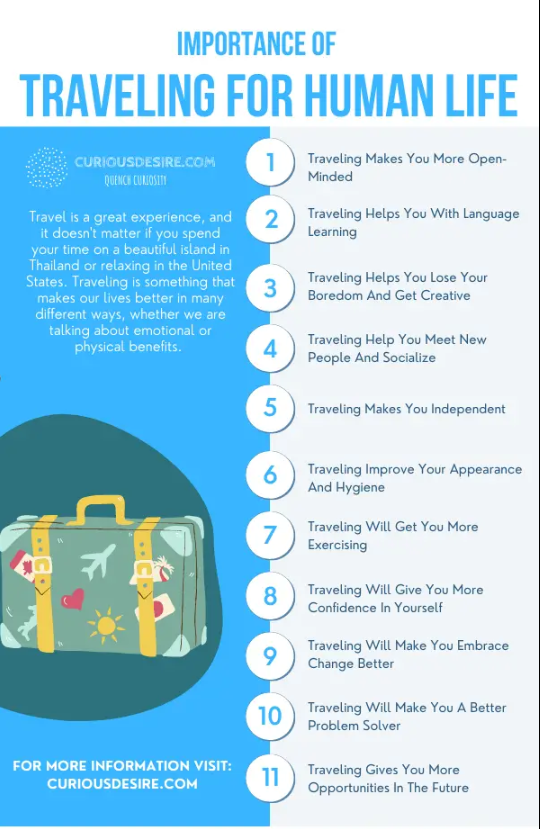
\includegraphics[width=0.45\textwidth]{/home/ada/Nextcloud2/risorse-next/mandes-esperto/importance_travel.png}
%\caption {Importance of traveling}


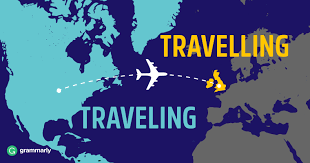
\includegraphics[width=0.5\textwidth]{/home/ada/Nextcloud2/risorse-next/mandes-esperto/english-movers_gitrepo/traveling.png}
\caption {American and English pronunciation}		
\vspace{3cm}

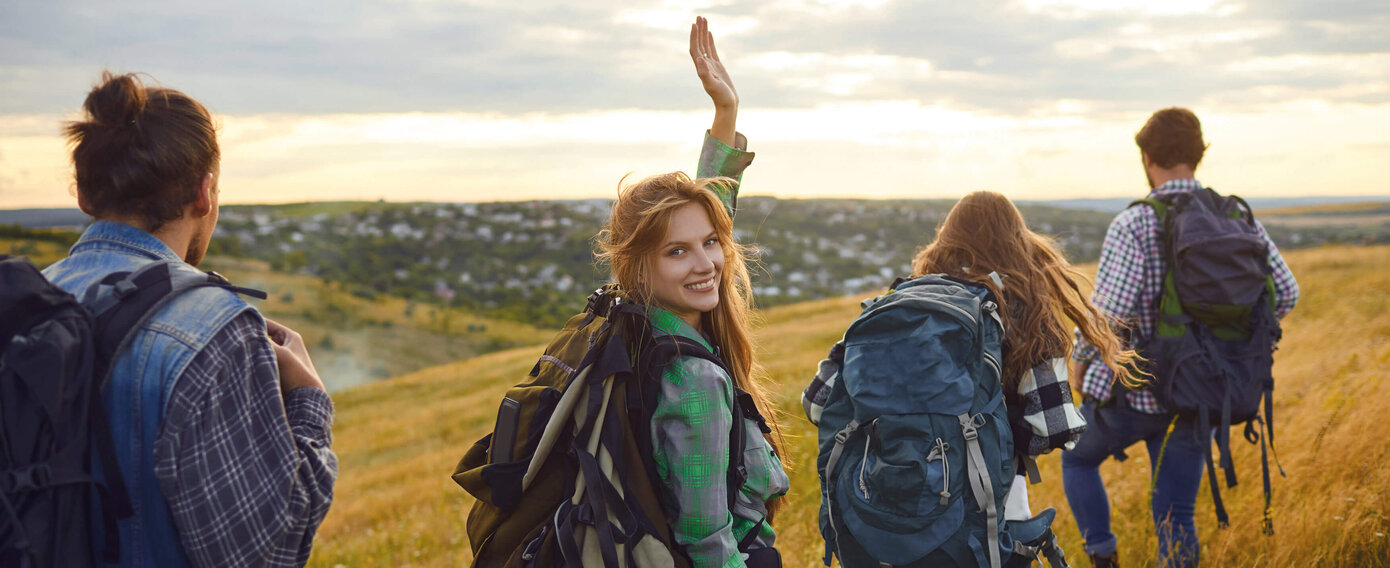
\includegraphics[width=0.5\textwidth]{/home/ada/Nextcloud2/risorse-next/mandes-esperto/english-movers_gitrepo/people-walking.jpg}
\caption {Benefit of travel}		

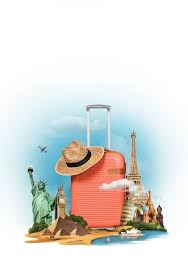
\includegraphics[width=0.5\textwidth]{/home/ada/Nextcloud2/risorse-next/mandes-esperto/english-movers_gitrepo/travel-baggage.jpeg}
%\caption {American and English}		

	\end{wrapfigure}
	
	
	
	
	\begin{dialogue}
		\speak{Alice} Hey John, are you excited for our trip to Paris next month?
		\speak{Bob} Definitely! I can't wait to see the Eiffel Tower in person.
		\speak{Alice} Oh no, I forgot my passport at home!
		\speak{Bob} Don't worry, we still have time before our flight. Let's go back and get it.
		\speak{Alice} Excuse me, where can I buy a ticket for the train?
		\speak{Bob} You can purchase one at the ticket office on the platform.
		\speak{Alice} I missed the last bus, how am I going to get home now?
		\speak{Bob} I can give you a ride, I'm heading in that direction anyway.
		\speak{Alice} Our flight is at 8am, what time should we leave for the airport?
		\speak{Bob} 30am.
		\speak{Alice} We're finally here, let's check-in to our hotel and rest.
		\speak{Bob} Sounds good, I can't wait to take a hot shower and sleep on a comfortable bed.
		\speak{Alice} I heard there's a famous landmark nearby, do you want to go see it?
		\speak{Bob} Definitely, let's put it on our itinerary for tomorrow.
		\speak{Alice} This museum is so interesting, I could spend hours here.
		\speak{Bob} Me too, there's so much to see and learn about.
		\speak{Alice} Can we join the city tour and explore the town together?
		\speak{Bob} Sure, that sounds like a fun way to see the sights.
		\speak{Alice} I want to buy a souvenir for my family, do you know any good shops?
		\speak{Bob} There's a market a few blocks away, they have a great selection of souvenirs.A I can't believe we're about to go bungee jumping, it's going to be an adventure!
		\speak{Bob} I know, I'm so nervous but excited at the same time.
		\speak{Alice} Let's rent a car and drive around the countryside to explore.
		\speak{Bob} That's a great idea, we can stop and take in the scenic views along the way.
		\speak{Alice} I've never been to a foreign country before, I'm a bit nervous.
		\speak{Bob} Don't worry, I'll be with you the whole time. Plus, it's always fun to try new things.
		\speak{Alice} We have to go through customs before we can enter the country.
		\speak{Bob} I hope there won't be a long line, I hate waiting in queues.
		\speak{Alice} Can you read a map? I think we're lost.
		\speak{Bob} Let me take a look. Yes, I can navigate us back on track.
		
		
		
	\end{dialogue}
	
\end{minipage}


\iffalse
\subsection*{Young Globetrotters: Tips for Embracing Unique Cultures}


Traveling when you're young is the BEST, but it's more than just epic selfies and cool food. The real magic is experiencing cultures different from your own. Here's how to make it awesome:
\begin{enumerate}
	
	\item{ Ditch the Guidebook Mentality: Before you go, research the basics but resist planning every detail. Leave room to get lost, wander off the tourist map, and stumble on those hidden gems!}
	\item{ Hello? Hola? Bonjour!: Learn a few key phrases in the local language. Even a basic "please" and "thank you" shows respect and opens doors.}
	\item{ Taste the Adventure: Eat where the locals eat! Street food, bustling markets – these are where you'll find the authentic flavors. Be bold, even if you don't recognize anything on the menu.}
	\item{ People Power: Talk to people! Locals, other travelers, anyone. Ask questions, learn their stories. You'll see the place through their eyes, not just a camera lens.}
	\item{ Respect is Key: Remember, you're a visitor. Dress appropriately, learn local customs, and be mindful of your impact. Travel is about exchange, not just taking.}
\end{enumerate}


So there you go! Embrace the unexpected and remember, the best souvenirs are the experiences that change how you see the world.
\vspace{1cm}
\begin{question}
	\textbf{Which tips do you find more valuable? Which one do you apply?}
\end{question}

\vspace{4cm}

\begin{figure}[htb]
	\centering
	\includegraphics[width=0.8\textwidth]{/home/ada/Nextcloud2/risorse-next/istockphoto-694356140-612x612-singapore.jpg}
	\caption {Landscape of Singapore}
\end{figure}

\fi 
	
\end{document}